\documentclass{article}
\usepackage[margin=0.8in]{geometry} % Set margins to 0.8 inch
\usepackage{graphicx} % Required for inserting images
\usepackage{hyperref}
\usepackage{tabularx}
\usepackage{amssymb}
\usepackage{float}
\usepackage{listings}
\usepackage{xcolor}

\lstset{
  basicstyle=\ttfamily\footnotesize,
  breaklines=true,
  breakatwhitespace=true,
  frame=single,
  numbers=left,
  numberstyle=\tiny,
  keywordstyle=\color{blue},
  commentstyle=\color{gray},
  stringstyle=\color{red},
  tabsize=4,
  captionpos=b,
  literate={_}{\_}1  % <-- add this line
}

\setlength{\parindent}{0pt}

\title{
    \Huge \textbf{Self-Balancing Robot}

    \vspace{100px}

    \large Course: ELEC 391 201 2024W2 \\[1em]
    \large Authors: Team B-17 (Tomaz Zlindra, Muntakim Rahman, Xianyao Li) \\[1em]
    \large Instructors: Dr.\ Joseph Yan and Dr.\ Cristian Grecu \\[1em]
    \large Submission Date: April 13th, 2025 \\
}

\date{} % Remove default date

\begin{document}

\pagenumbering{gobble} % Suppress page numbering for the title page
\maketitle

\newpage % Start numbering after title page
\pagenumbering{arabic} % Restart numbering at 1

\tableofcontents % Generate Table of Contents

\newpage % Start main content

\section{Introduction}

• Description of the engineering problem or challenge
• Background context and any relevant history

\section{Requirements, Specifications and Constraints}
• It's helpful to list these in a table or enumerated, (e.g. R1, R2, etc.) so this can be treated as of checklist of
requirements that must be tested as detailed in the Verification and Validation section.
\subsection{Functional Requirements}

The table below (\ref{tab:functional_requirements}) lists all the functional requirements of the robot

\begin{table}[H]
    \centering
    \renewcommand{\arraystretch}{1.3} % Increase row height for readability
    \begin{tabularx}{\textwidth}{|c|X|c|}
        \hline
        \textbf{ID} & \textbf{Requirement Description} & \textbf{Priority} \\
        \hline
        FR1 & The robot must balance on a flat surface by controlling the DC motors. & Core \\
        \hline
        FR2 & The robot must maintain balance while driven externally on a flat surface. & Core \\
        \hline
        FR3 & The robot must maintain balance while turning at a reasonable speed. & Core \\
        \hline
        FR4 & The robot must move forward and backward under external control. & Core \\
        \hline
        FR5 & The robot must be controlled via Bluetooth with four directional commands. & Core \\
        \hline
        FR6 & The robot must maintain balance on a track with up to 15 degrees of incline. & Core \\
        \hline
        FR7 & The distance sensor must detect obstacles within 5-50 cm and stop the robot within 20 cm. & Additional Feature \\
        \hline
        FR8 & The color sensor must be able to detect at least red, green and blue colors & Additional Feature \\
        \hline
        FR9 & The RFID module must authenticate an RFID tag within 1 second to prevent unauthorized operation. & Additional Feature \\
        \hline
        FR10 & The Raspberry Pi Zero must process and transmit a camera feed at least 1 FPS. & Additional Feature \\
        \hline
    \end{tabularx}
    \caption{Functional Requirements of the Self-Balancing Robot}
    \label{tab:functional_requirements}
\end{table}

\subsection{Performance Requirements}
Metrics for performance such as speed, efficiency, capacity, etc.
\subsection{Constraints}
(financial, temporal, material, environmental, standards and regulations to follow, etc.)

\section{Conceptual Design}
High level functional diagram/architecture of the overall system.

\subsection{High-level Functional Diagram}

\begin{figure}[H]
    \centering
    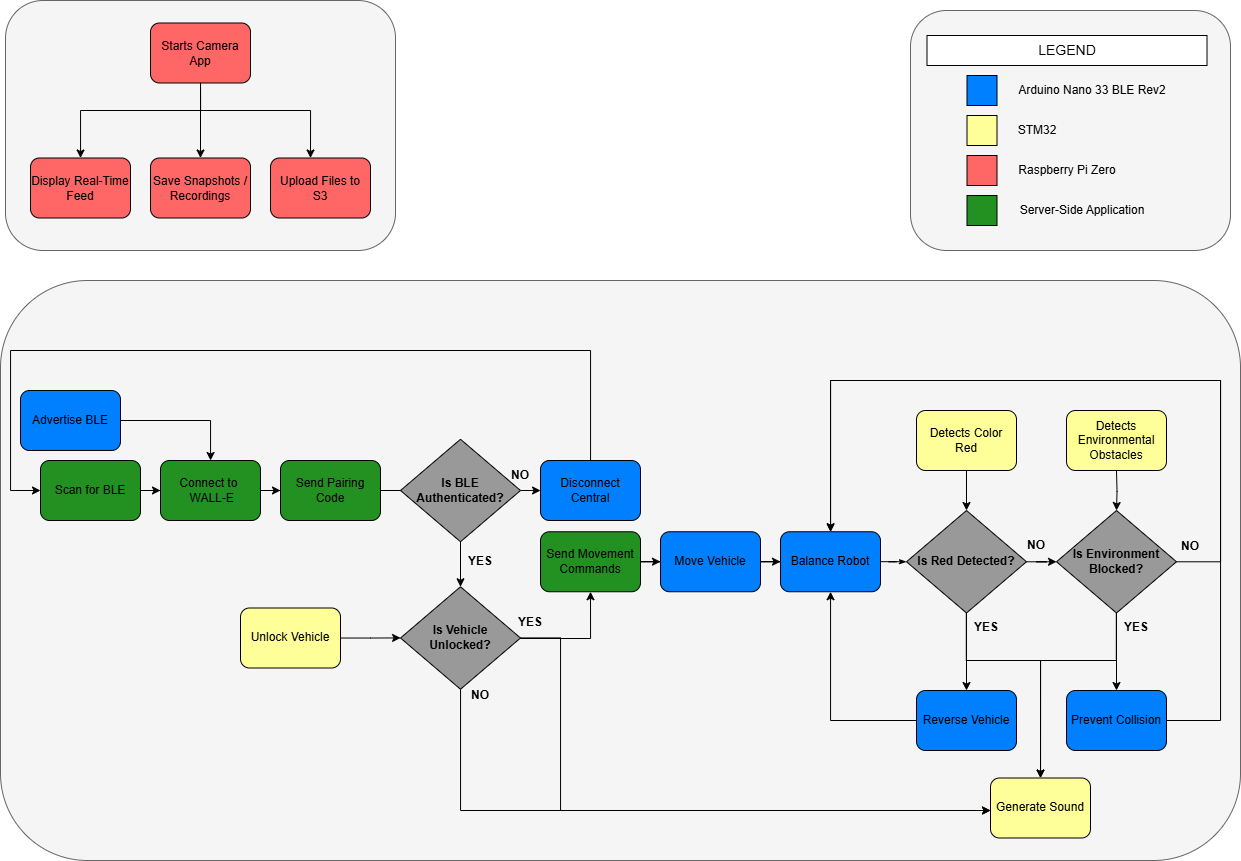
\includegraphics[width=1\textwidth]{Figures/Functional_Diagram.png}
    \caption{High-level Functional Diagram}
    \label{fig:functional_diagram}
\end{figure}

\begin{minipage}{\linewidth}
    The functional diagram in Figure~(\ref{fig:functional_diagram}) highlights our system-design for enforcing secure access of the robot with
    \textbf{RFID} and \textbf{Bluetooth Low Energy (BLE)}. We prevent users from balancing or moving the robot without the required authentication. Once successful,
    the firmware was programmed to prioritize safe operation of the robot, while accounting for environmental factors such as distance and color detection. \\
\end{minipage}

\subsection{Architecture Diagram}

\begin{figure}[H]
    \centering
    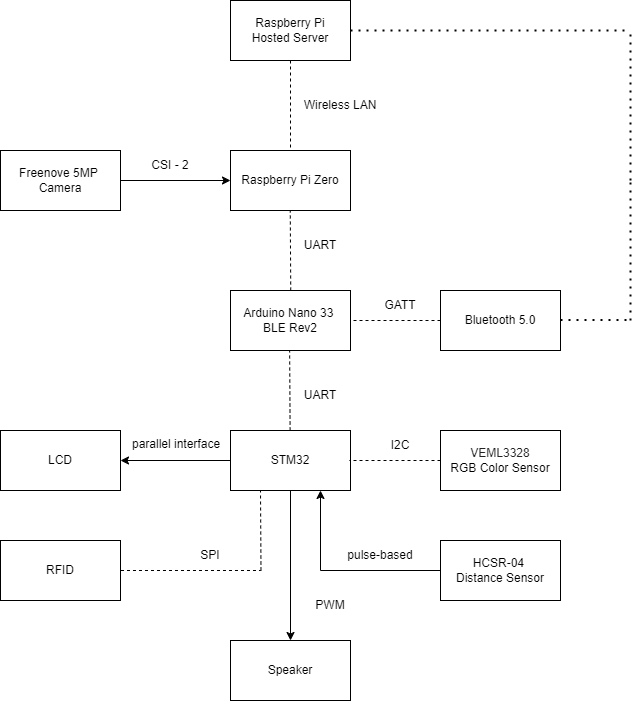
\includegraphics[width=0.7\textwidth]{Figures/Architecture_Diagram.png}
    \caption{Architecture Diagram}
    \label{fig:architecture_diagram}
\end{figure}

\textbf{This might need to be updated. We should also add some text to explain what is going on}

\section{Subsystem Design}
Detailed description and schematics for key subsystems \\
Include electrical, mechanical, structural, or process-related subsystems as appropriate


\subsection{Mechanical Design}

\textbf{still unsure of what to write in this section, possibly how the motors/sensors were mounted, materials we used,etc.}

\subsection{Structural Design}

\textbf{Explain why the third layer is higher rather than lower. Explain why no weight was added anywhere else. A part of this section should also include why the sensors and modules were mounted the way they were done}

\subsection{PID Modeling and Simulation}

\textbf{Measuring Robot Parameters} \\

Write here a small section on how the robot mass was calculated, torque from motors, etc.

\textbf{Transfer Function} \\

% \begin{figure}[H]
%     \centering
%     \includegraphics[width=0.6\textwidth]{Figures/pid_control_diagram.png} % Adjust width as needed
%     \caption{PID Control Diagram}
%     \label{fig:pid_control_diagram}
% \end{figure}

The exact transfer function used (reference the PhD study). There should be an image showing the exact control diagram here too

\textbf{MATLAB PID Simulation} \\

Just the matlab stuff and have a code listing in the appendix

\subsection{Arduino Nano 33 BLE Sense Rev2}

\begin{figure}[H]
    \centering
    \includegraphics[width=0.6\textwidth]{Figures/arduino.jpg} % Adjust width as needed
    \caption{Arduino Nano 33 BLE Sense Rev2}
    \label{fig:arduino}
\end{figure}

\begin{minipage}{\linewidth}
    The \textbf{Arduino Nano 33 BLE Sense Rev2}  is a compact and powerful microcontroller board
    designed for low-power applications. It features the Nordic \textbf{nRF52840} chipset,
    which supports \textbf{BLE} communication, includes a range of built-in sensors,
    including a 9-axis IMU (accelerometer, gyroscope, and magnetometer).
    These integrated features make it well-suited for IoT, sensor-based applications, and portable devices. \\

    This made it the ideal choice for our self-balancing robot project and was responsible for many of the core features.
    It integrated key core components in this project, particularly the IMU and the \textbf{BLE} module. \\
\end{minipage}


\subsubsection{Arduino IDE}

\begin{minipage}{\linewidth}
    The \textbf{Arduino IDE} was integral in quickly testing new firmware changes to the board with built-in compilation and flashing tools.
    The extensive library support significantly streamlined the development process, reducing the need for bare metal programming and allowing us to focus on the functionality.
\end{minipage}


\subsection{Angle Measurement}
\label{sec:angle}

\begin{figure}[H]
    \centering
    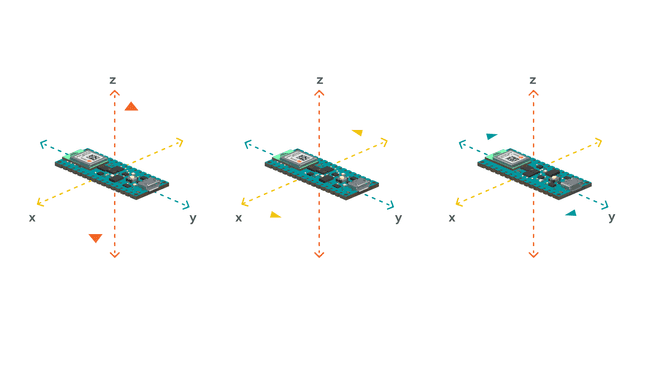
\includegraphics[width=0.6\textwidth]{Figures/imu.png} % Adjust width as needed
    \caption{IMU}
    \label{fig:imu}
\end{figure}

\begin{minipage}{\linewidth}
    The \textbf{Inertial Measurement Unit (IMU)} was a critical component of the microcontroller for measuring velocity, orientation, and
    gravitational forces. This enabled the tracking of motion and orientation of the \textbf{Arduino} in three-dimensional space.
\end{minipage}

\subsubsection{IMU Sensors}
\begin{minipage}{\linewidth}
    We used the accelerometer to measure linear acceleration and the gyroscope to monitor rotational
    movement. Both of these sensors had advantages and disadvantages, as shown in Table~\ref{tab:imu_sensors}. \\

    By combining them, we ensured reliable and accurate angle measurements for optimized balancing in the control feedback loop.
\end{minipage}

\subsubsection{Complementary Filter}

% \begin{figure}[H]
%     \centering
%     \includegraphics[width=0.6\textwidth]{Figures/complementary_filter.png} % Adjust width as needed
%     \caption{Complementary Filter Feedback Diagram}
%     \label{fig:complementary_filter}
% \end{figure}

\begin{minipage}{\linewidth}
    The solution to combine the strengths of both sensors was to use a complementary filter,
    which combines the accelerometer and gyroscope readings with their respective normalized weights. \\

    Since the gyroscope provided a rough estimate of the angle change, this was essential for detecting quick movements. \\
\end{minipage}

The formula used for the complementary angle is:

\[
\theta_n = k(\theta_{n-1} + \theta_{g,n}) + (1-k)\theta_{a,n},
\]

where:
\begin{itemize}
    \item $\theta_n$ is the current complementary angle,
    \item $\theta_{n-1}$ is the previous complementary angle,
    \item $\theta_{g,n}$ is the current gyroscope angle,
    \item $\theta_{a,n}$ is the current accelerometer angle,
    \item $k$ is the normalized weight.
\end{itemize}

\begin{center}
    $\therefore$ From extensive testing, a value of $k = 0.95$ was selected. \\
\end{center}

\textit{
    Lower values of $k$ caused the noise from the accelerometer to become significant, leading to large oscillations and loss of balance.
    Similarly, increasing $k$ was avoided. The gyroscope bias would accumulate quickly (i.e., without a reference point)
    and cause the robot to lose balance.
}\vspace{0.5cm}

The code snippet for this exact implementation is demonstrated in Listing \ref{lst:arduino_angle_code}.

\subsection{Autonomous-Balancing}

\begin{minipage}{\linewidth}
    The most challenging part of this project was to implement the PID controller to balance the robot. Since we had closed-loop control,
    with the measured angle acting as feedback, it was crticial that we were able to act upon new measurements when determining the control signal. \\

    Initially, we attempted to implement these \textbf{Interrupt Service Routine (ISR)} to meet a designed control frequency of $20$ Hz.
    However, this proved to accumulate complications in firmware logic and was not able to provide the expected results. \\

    We ultimately designed a control loop, run in the main program. This followed the sequence shown in Figure~\ref{fig:control_loop_diagram}.
\end{minipage}

\begin{figure}[H]
    \centering
    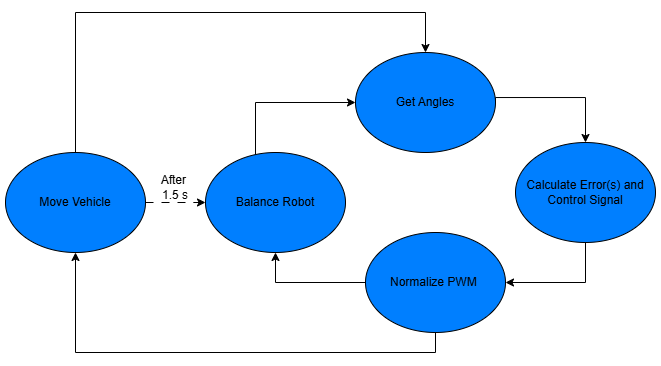
\includegraphics[width=0.75\textwidth]{Figures/Control_Loop_Diagram.png}
    \caption{Control Loop Diagram}
    \label{fig:control_loop_diagram}
\end{figure}

\begin{minipage}{\linewidth}
    This ensured that we were able to inject \textbf{PWM} signals to both motors, without the constraints typical of an \textbf{ISR}. At the same time,
    this ensured that the robot was acting upon the most recent measurements. \\

    The sign of the control signal determined whether to move the robot forward / backward to maintain balance.
\end{minipage}

\subsection{Movement}
\label{sec:movement}

\begin{minipage}{\linewidth}
    The robot was designed to move in four directions: \textbf{FORWARD, BACKWARD, LEFT, RIGHT}.
    As shown in Figure~\ref{fig:control_loop_diagram}, this was designed to be integrated into the control loop.  \\

    Balancing was the highest priority of the system at any given time. To move the robot, we injected noise into the system for a short period of time
    (i.e. $1.5$ seconds). After this, we returned to idle balancing to prevent the system from reaching a point of instability. \\
\end{minipage}

\subsubsection{Forward/Backward Movement}

\begin{minipage}{\linewidth}
    The logic for moving the robot forward and backward was very simple. It was a matter of adjusting the setpoint angle on either side of the "zero point".
    This induced movement in the indended direction (without sacrificing balance). \\
\end{minipage}

\subsubsection{Left/Right Movement}

\begin{minipage}{\linewidth}
    The logic for moving the robot left and right was slightly more complicated and involved
    software logic to interchangeable turn and balance the robot. This can be summarized as follows: \\
\end{minipage}

\begin{itemize}
    \item Every 3 iterations of control loop : balance robot
    \item If error angle $>$ allowable threshold (i.e. 0.8 degrees): balance robot
    \item Otherwise:
    \begin{itemize}
        \item To turn left: move left motor $CW$ and right motor $CCW$, with \textbf{PWM} adjusted by scale factor $0.6$
        \item To turn right: move left motor $CCW$ and right motor $CW$,  with \textbf{PWM} adjusted by scale factor $0.5$
    \end{itemize}
\end{itemize}

\subsection{Bluetooth Control}

\begin{minipage}{\linewidth}
    The robot was controlled via the \textbf{Arduino's} \textbf{Bluetooth Low Energy (BLE)} capabilities.
    The firmware was developed such that new connections need to be authorized by successfully transmitting
    the correct pairing code. This follows the workflow shown in Figure~\ref{fig:functional_diagram}. \\

    In order to send movement commands, the connection and authentication process must be successfully complete to ensure secure access. A key
    part of this process was to provide the expected pairing code to the microcontroller. \\
\end{minipage}

\begin{figure}[H]
    \centering
    \fbox{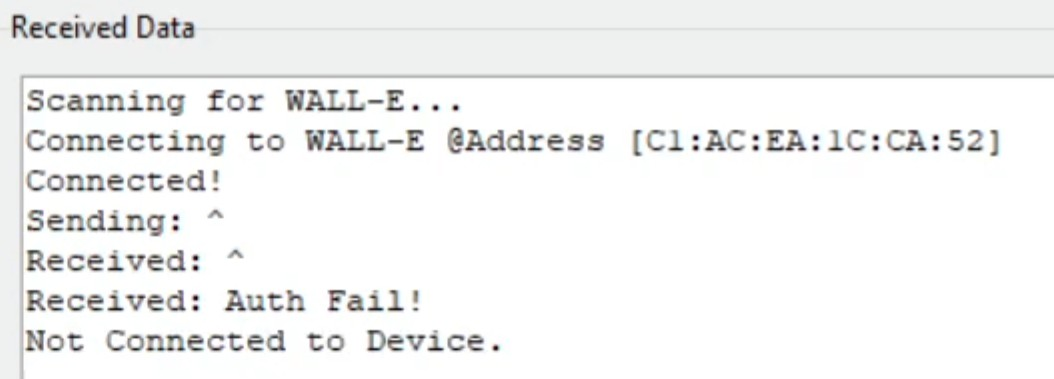
\includegraphics[width=0.5\textwidth]{Figures/Unauthorized_Connection.jpg}}
    \caption{Unauthorized Bluetooth Connection}
    \label{fig:bluetooth_unauthorized}
\end{figure}

\begin{minipage}{\linewidth}
    If unsuccesful, the robot would immediately disconnect and await an authorized user as shown in Figure~\ref{fig:bluetooth_unauthorized}. \\

    The firmware is also designed such that movement commands are placed on a lower priority. Since \textbf{BLE} can be computationally expensive,
    we polled for new commands every $100$ ms in the main loop. This was done to ensure that the control functionality is placed at highest priority,
    and we can account for the infrequent nature of user driven commands.
\end{minipage}

\subsubsection{Robot Driver App}

\begin{minipage}{\linewidth}
    We developed a \textbf{Flask} application, which used \texttt{GET/POST} request \textbf{HTTP} methods
    to asynchronously request device information from the \textbf{HTML DOM} elements and send commands to the
    \textbf{Arduino} microcontroller. \\

    This application was run from our computer and temporarily hosted to the Internet using the \textbf{ngrok} tool.
    This enabled us to access the robot via public URL from other devices (including smartphones).
\end{minipage}\vspace{0.5cm}

\begin{figure}[H]
    \centering
    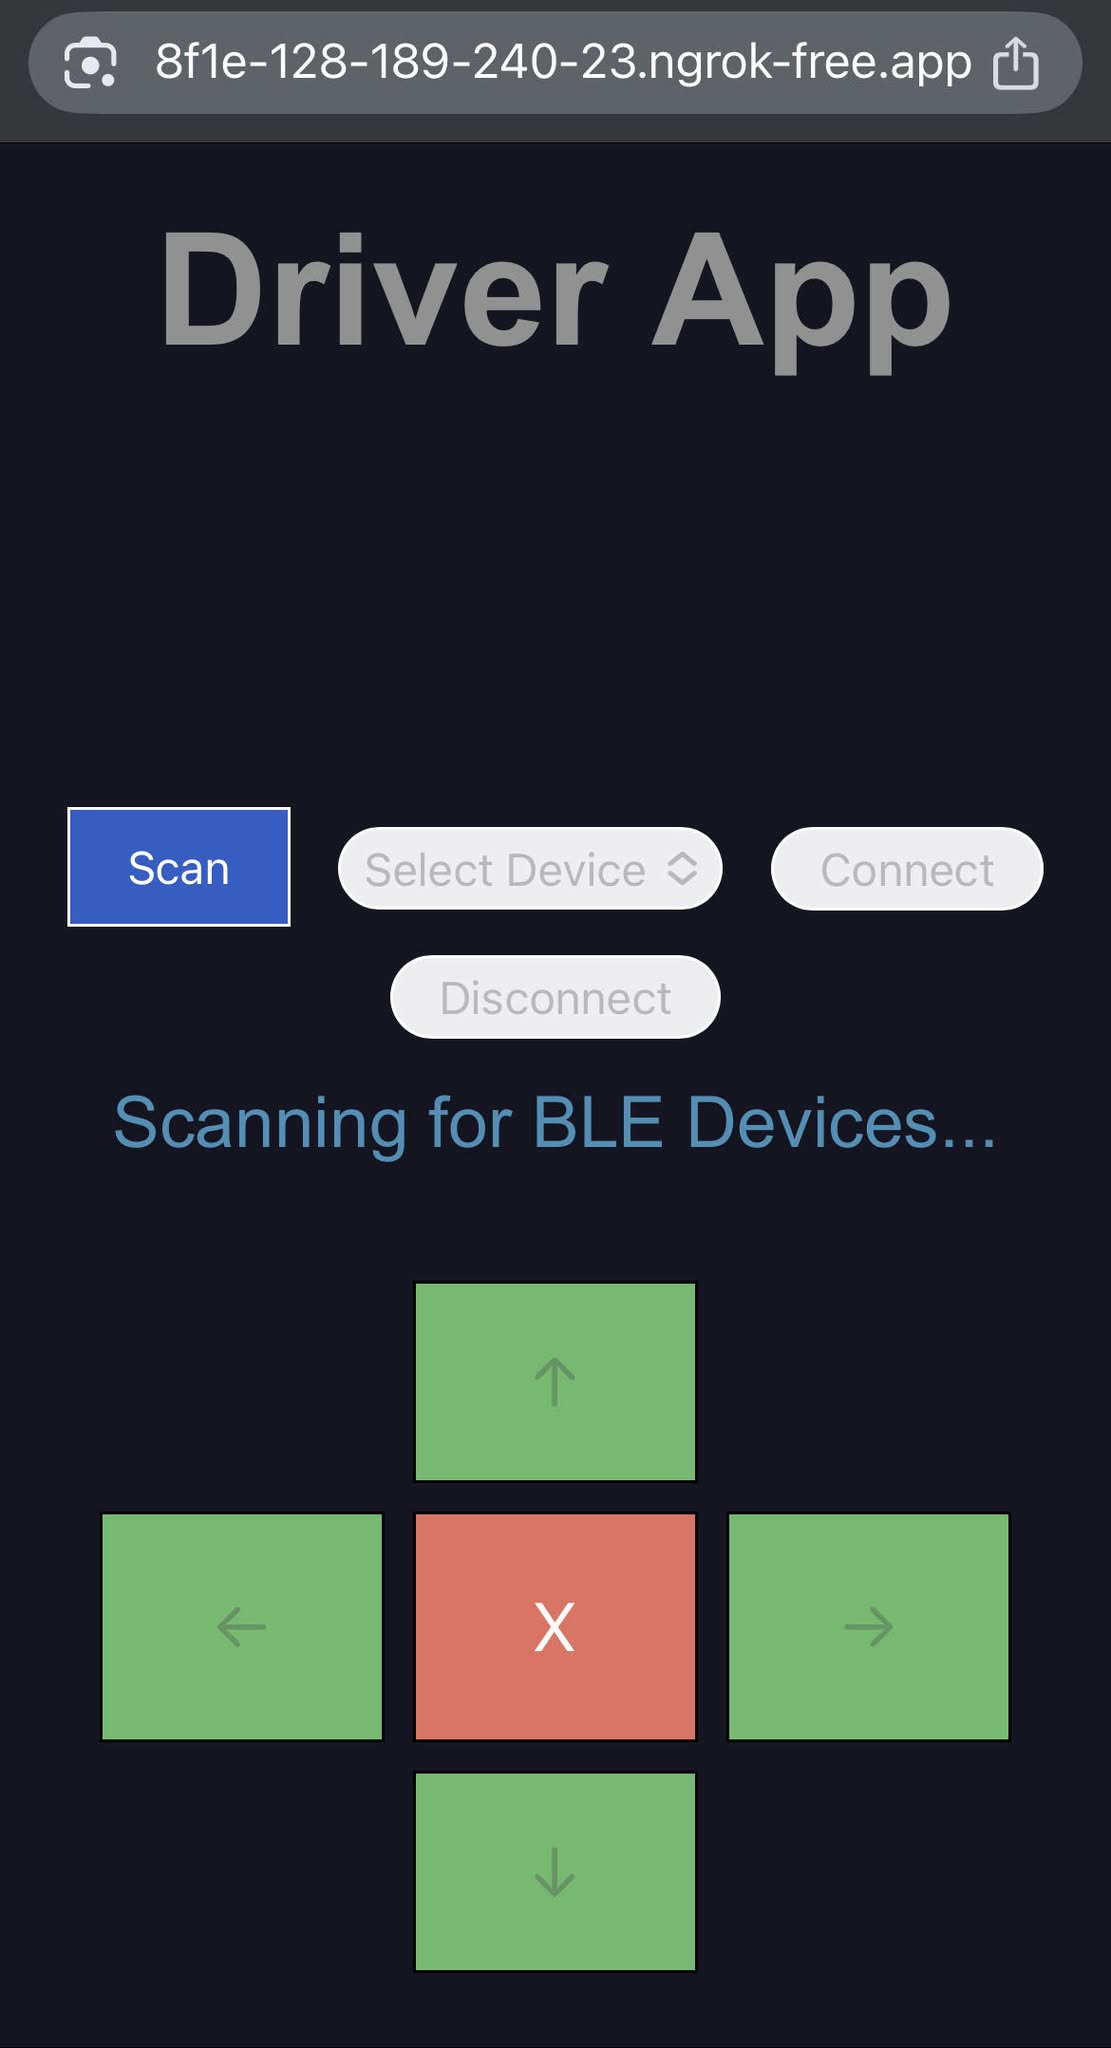
\includegraphics[width=0.25\textwidth]{Figures/Robot_Driver_App.jpg}
    \caption{Robot Driver App on iPhone 14}
    \label{fig:ble_app}
\end{figure}

\begin{minipage}{\linewidth}
    The \textbf{Flask} application had the expected pairing code programmed in the source code such that users can easily connect to and control the robot.
    We programmed the \texttt{DRIVE, LEFT, RIGHT, BACK} commands to correspond to specific bytes to be transmitted via \textbf{BLE}. \\
\end{minipage}

\begin{center}
    This is shown in the code snippet in Listing \ref{lst:driver_app_code} in the Appendix.
\end{center}

\subsection{STM32L051K8T6 Microcontroller}
\label{sec:stm32}

\begin{figure}[H]
    \centering
    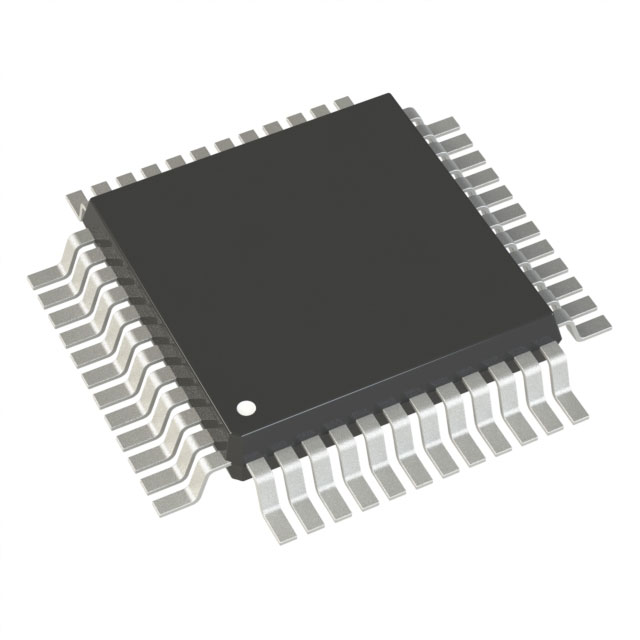
\includegraphics[width=0.5\textwidth]{Figures/stm32.jpg} % Adjust width as needed
    \caption{STM32L051K8T6 Microcontroller}
    \label{fig:stm32}
\end{figure}

The STM32L051K8T6 is a low-power microcontroller from STMicroelectronics, part of the STM32L0 series. It features an ARM Cortex-M0+ core running at up to 32 MHz, with 64 KB of flash memory and 8 KB of SRAM. The microcontroller offers a variety of peripherals, including I2C, SPI, UART, ADC, and GPIO, along with multiple low-power modes. For our project, this microcontroller was used to interface with the HC-SR04 (section \ref{sec:distancesensor}), TCS34725 (section \ref{sec:colorsensor}), RC522 (section \ref{sec:rfidsensor}) and the CEM-1202 (section \ref{sec:speaker}) modules.

\

Due to the limited number of peripherals on the STM32L051K8T6 microcontroller comprising 2 USART ports, 1 I$^2$C, and 1 SPI interface, along with only 27 available I/O pins—we were required to carefully allocate communication protocols to each sensor (I$^2$C for the color sensor and SPI for the RFID sensor). We opted not to use UART to maintain simplicity and efficiency. Out of the 27 I/O pins, we utilized approximately 20. It is worth noting that although USART is enabled in the configuration (as shown in Figure~\ref{fig:stm32_pinout_zoomed_in}), it was never used in the implementation.


\begin{figure}[H]
    \centering
    \begin{minipage}[b]{0.45\textwidth} % Adjust width as needed
        \centering
        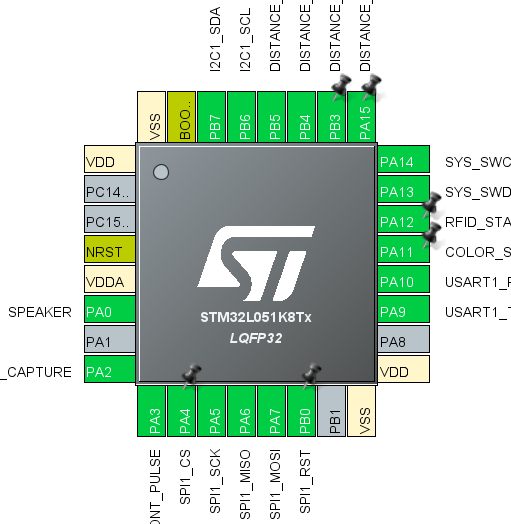
\includegraphics[width=8\textwidth, height=0.4\textheight, keepaspectratio]{Figures/stm32_pinout_in.png}
        \caption{Zoomed In Pinout}
        \label{fig:stm32_pinout_zoomed_in}
    \end{minipage} \hfill
    \begin{minipage}[b]{0.48\textwidth} % Adjust width as needed
        \centering
        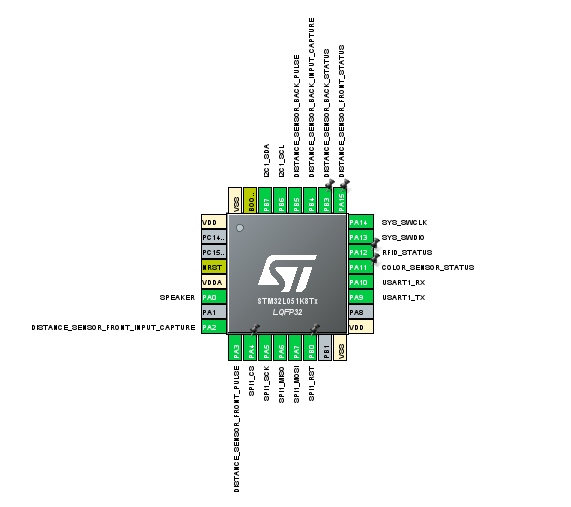
\includegraphics[width=\textwidth, height=0.4\textheight, keepaspectratio]{Figures/stm32_pinout_out.png}
        \caption{Zoomed Out Pinout}
        \label{fig:stm32_pinout_zoomed_out}
    \end{minipage}
\end{figure}

To streamline the firmware development process for the STM32, we utilized the STM32Cube IDE, provided by STMicroelectronics. This development environment facilitated faster progress by offering built-in tools and libraries, allowing us to focus on application logic rather than dealing with bare-metal programming.



\subsection{HC-SR04 Ultrasonic Ranging Module}
\label{sec:distancesensor}

\begin{figure}[H]
    \centering
    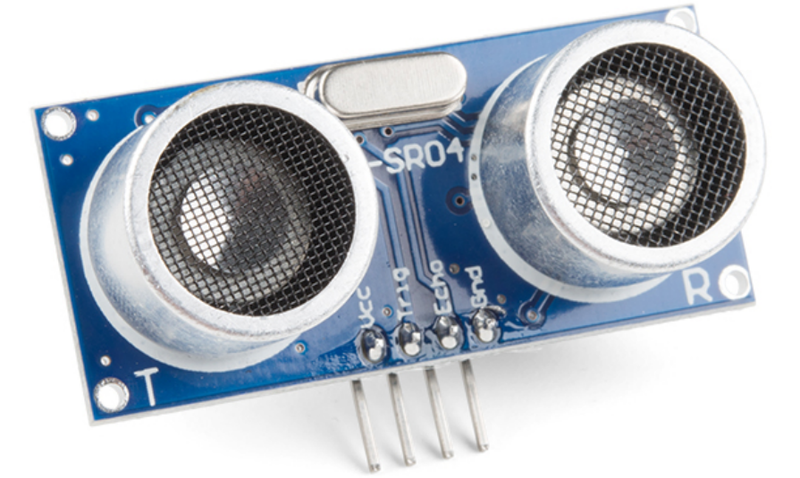
\includegraphics[width=0.6\textwidth]{Figures/distancesensor.png} % Adjust width as needed
    \caption{HC-SR04 Ultrasonic Ranging Module}
    \label{fig:distancesensor}
\end{figure}

The \textbf{HC-SR04} is an ultrasonic distance measurement module commonly used in embedded systems for sensing proximity to objects. It operates by emitting an ultrasonic pulse from its transmitter and measuring the time it takes for the pulse to reflect off a nearby surface and return to the receiver. The module communicates via a simple TTL interface, requiring a 'trigger' signal to start the measurement and an 'echo' signal to indicate when the reflected pulse is received. By calculating the time interval between the trigger and echo signals, the distance to the object can be determined.

\

Firmware for interfacing with this module was developed on the \emph{STM32L051} microcontroller, chosen for its ease of integration via HAL libraries and to offload processing from the Arduino Nano. Since the STM32 also handled other peripherals, efficient use of its timer channels with interrupts was essential to avoid overloading the main control loop.

\

The timer was configured with a prescaler of 31 (yielding a 1MHz timer frequency) to provide microsecond-level precision. One channel was set to PWM mode with a 10-cycle pulse (10$\mu$s) to drive the Trigger pin. Another channel was configured in input capture mode, connected to the Echo pin. This setup allowed interrupts to be triggered on both rising and falling edges of the Echo signal, enabling precise capture of timer values at each transition. By handling these events in interrupt service routines, the CPU remained free to execute other tasks concurrently with the distance measurement process.

\

A code sample for the firmware implementation of input capture interrupt are shown in Listing \ref{lst:stm32_distancesensor_code} in the Appendix. More information about input capture mode and its implementation can be found on this site, \href{https://community.st.com/t5/stm32-mcus/how-to-use-the-input-capture-feature/ta-p/704161}{here}.

\subsection{TCS34725 Light-to-Digital Sensor}
\label{sec:colorsensor}
\begin{figure}[H]
    \centering
    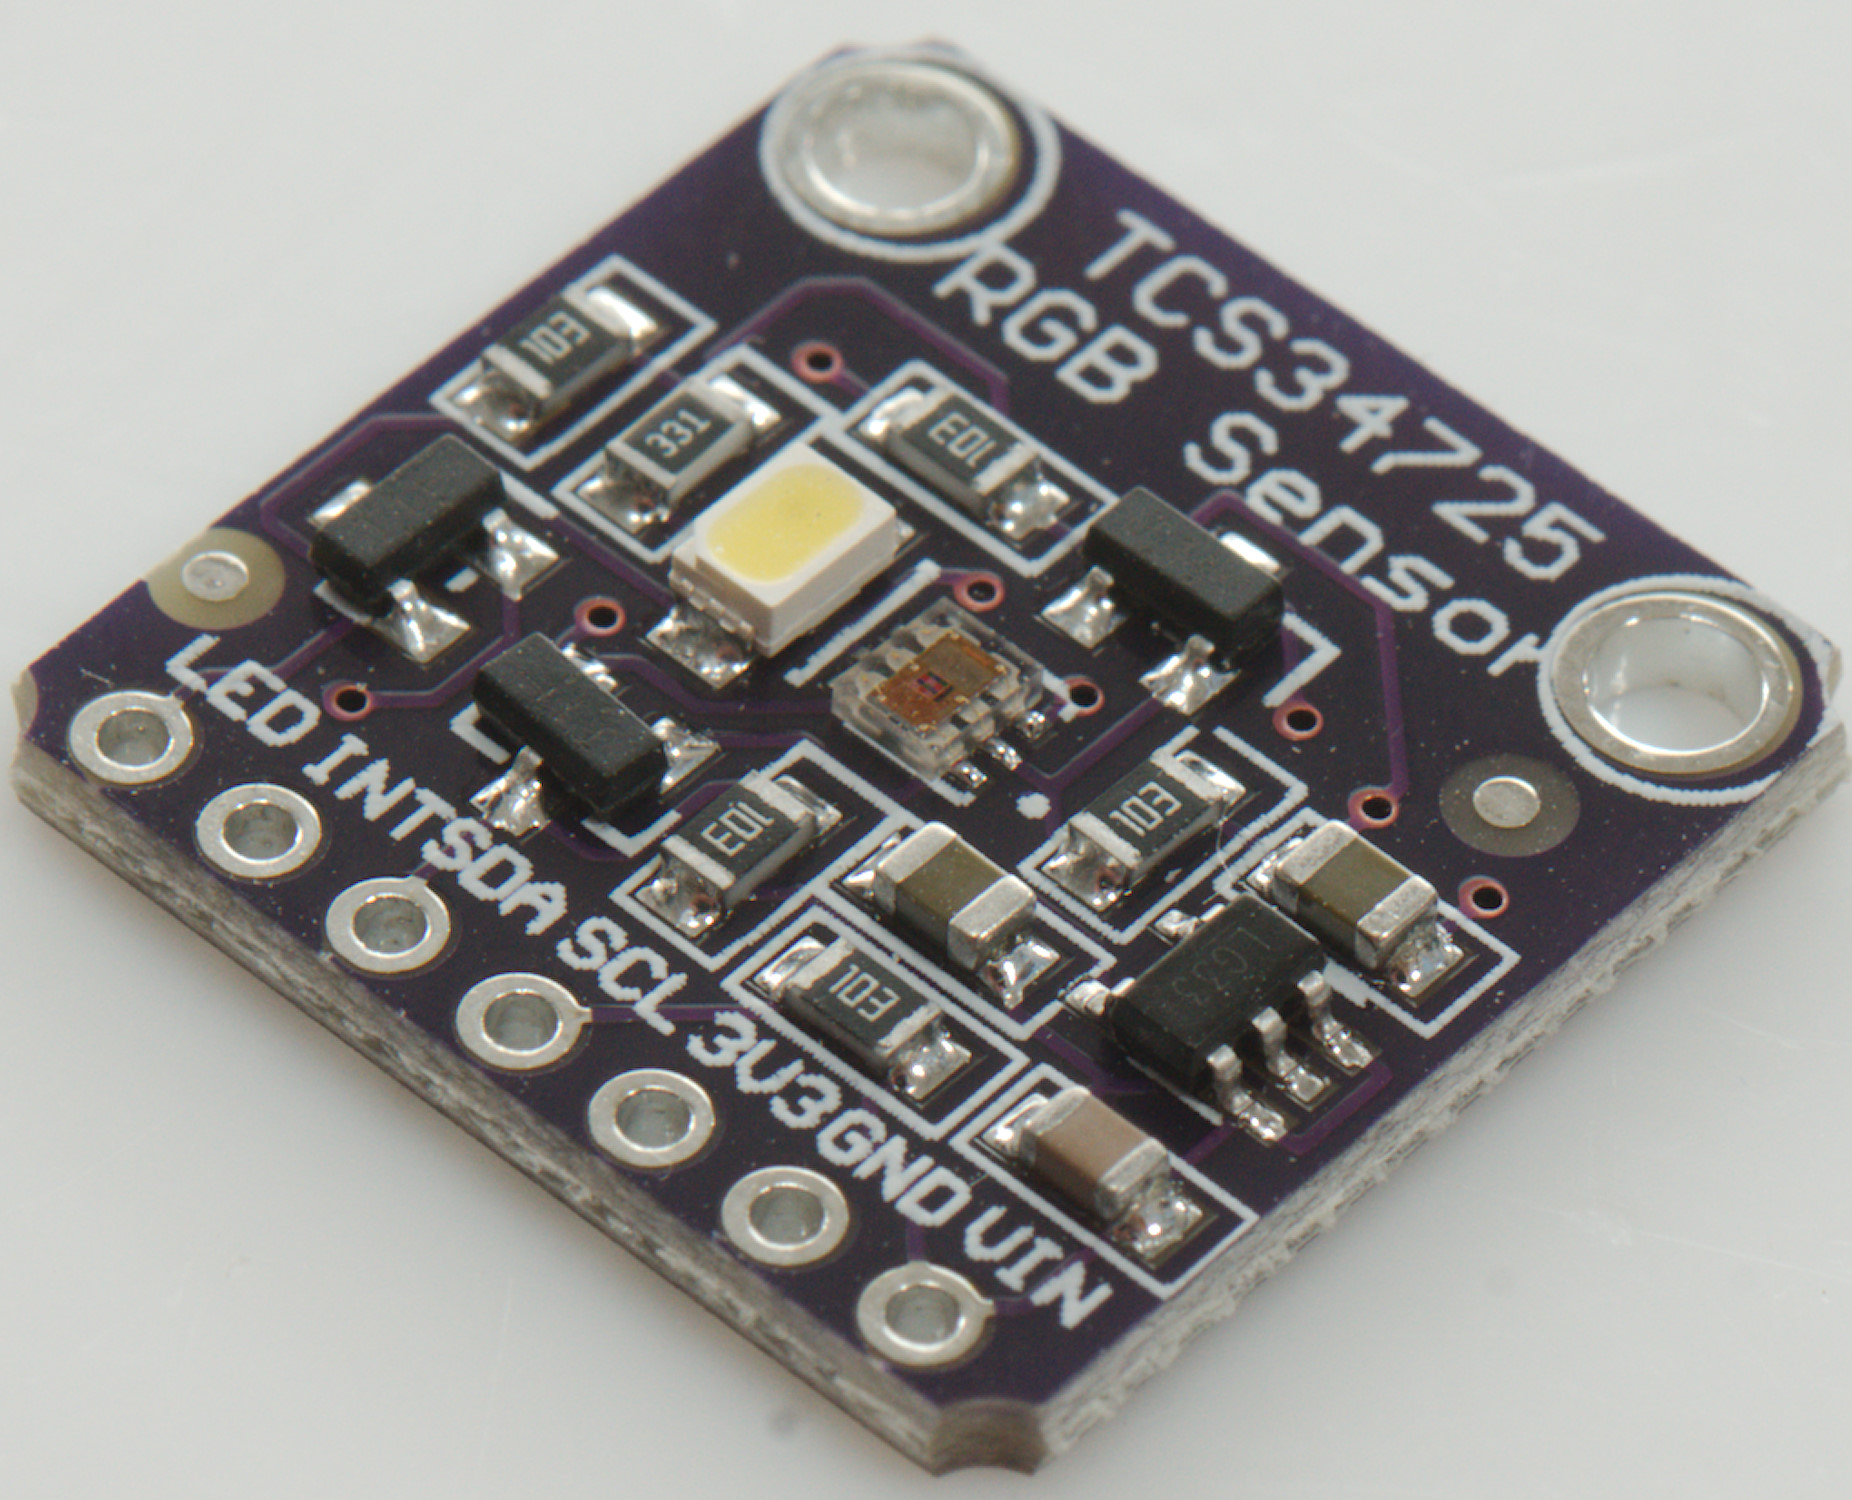
\includegraphics[width=0.6\textwidth]{Figures/colorsensor.jpg} % Adjust width as needed
    \caption{TCS34725 Light-to-Digital Sensor}
    \label{fig:colorsensor}


\end{figure}

The \textbf{TCS34725} Color Sensor Module was responsible for detecting the color composition of a surface by measuring the intensity of red, green, blue, and clear light. It communicates via an I$^2$C interface and features an integrated IR filter to improve color accuracy under varying lighting conditions. When illuminated, typically by its onboard white LED, the sensor captures reflected light and provides digital values corresponding to each color channel. These values can be used to determine the overall color or detect specific color patterns in an environment.

\

This module was implemented on the \emph{STM32L051} microcontroller instead of the Arduino Nano to reduce unnecessary clock cycle usage associated with I\textsuperscript{2}C communication. This decision allowed more processing time to be allocated to tasks such as maintaining the balance of the robot and BLE communication. The STM32 HAL libraries simplify I\textsuperscript{2}C communication, as demonstrated in Listing~\ref{lst:stm32_colorsensor_code}. Although we could've used DMA or interrupts for this module, we decided to not make it unnecessarily complicated and just left it in the main loop, as is.

\

The \texttt{ColorSensor\_Handle} function is called within the main control loop. It reads the values from each color channel register (16 bits) and determines the most dominant color. If the red channel is the most prominent, the speaker is triggered to notify the user of the sensor's detection.


\subsection{RC522 Contactless Reader IC}
\label{sec:rfidsensor}
\begin{figure}[H]
    \centering
    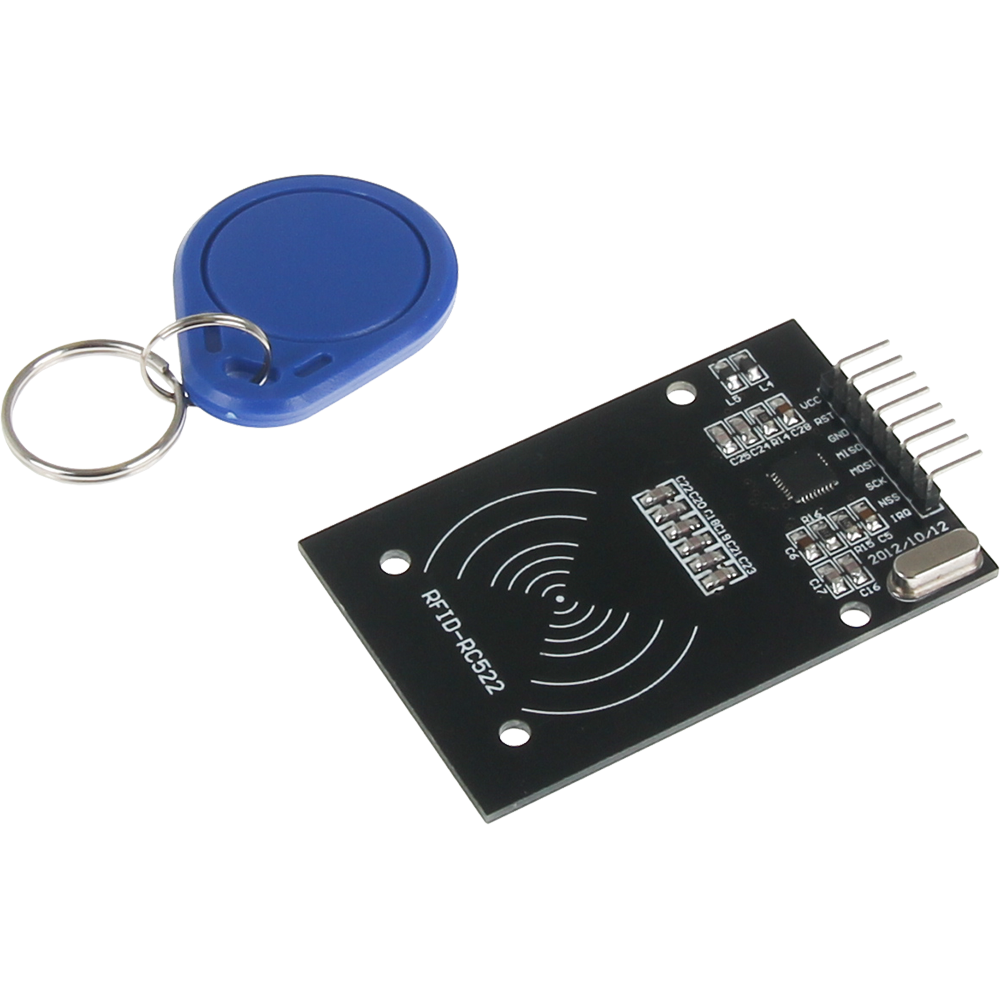
\includegraphics[width=0.6\textwidth]{Figures/rfidsensor.png} % Adjust width as needed
    \caption{RC522 Contactless Reader IC}
    \label{fig:rfidsensor}


\end{figure}

The \textbf{RC522} RFID Module was responsible for detecting and reading passive RFID tags using radio frequency communication at 13.56MHz. It operates over an SPI interface, allowing for fast and efficient data exchange with a microcontroller. When a tag enters the RF field generated by the module’s antenna, the RC522 initiates a handshake protocol and reads the tag’s unique identifier (UID) stored in its internal memory. This UID can then be used for identification or authentication purposes in embedded systems.

\

This module was also interfaced with the \emph{STM32L051} microcontroller, primarily due to its ease of use and to offload processing responsibilities from the Arduino Nano. Given the large number of configuration registers required by the RC522 chip, an existing \href{https://github.com/Hamid-R-Tanhaei/RFID-MIFARE-RC522-ARM-STM32/blob/main/Firmware_stm32f103zct6/Src/MFRC522.c}{STM32 implementation} was used as a reference, and its library was integrated into our firmware. The remaining logic specific to our application is shown in Listing \ref{lst:stm32_rfidsensor_code} in the Appendix.

\subsection{CEM-1302 Speaker/Buzzer}
\label{sec:speaker}
\begin{figure}[H]
    \centering
    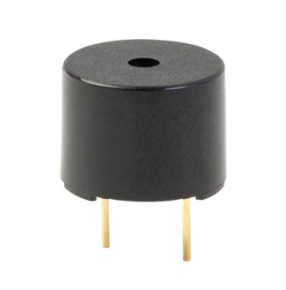
\includegraphics[width=0.6\textwidth]{Figures/speaker.png} % Adjust width as needed
    \caption{CEM-1302 Speaker/Buzzer}
    \label{fig:speaker}


\end{figure}

The \textbf{CEM-1302} speaker is a compact piezoelectric buzzer designed to produce audible tones. It operates by generating sound through the vibration of a diaphragm when an AC signal is applied. This module is commonly used in embedded systems to provide simple, high-pitched alerts or notifications.

\

The speaker was driven by the \emph{STM32L051} microcontroller, utilizing timers in PWM mode. Given that the resonant frequency of the buzzer is approximately 2.048 kHz, we configured the timer with a prescaler of 31 (32 - 1) to achieve an overflow frequency of 1 MHz. With this setup, we set the capture compare value to 488 and the pulse width to 244, resulting in a PWM signal that generates a frequency close to 2.048 kHz with a 50\% duty cycle.

\

This buzzer was used to provide feedback for the following events:
\begin{itemize}
    \item RFID: Indicating successful and unsuccessful RFID card scans
    \item Ultrasonic Sensor: Alerting when the distance between the robot and an object is too small
    \item Color Sensor: Signaling when the color sensor detects a predominantly red color
\end{itemize}

When any of these events occurred, the speaker would either beep, or stay on, depending on the scenario. Code for the setup can be seen in Listing \ref{lst:stm32_speaker_code}. GPIO pins for these events were used to communicate with the Arduino Nano rather than UART for communication, as its higher overhead
and slow speed was deemed unfit for the task at hand.

\subsection{Raspberry Pi Zero 2 W}

The \textbf{Raspberry Pi Zero 2 W} is an affordable single-board computer designed for
embedded systems and IoT applications. We leveraged its camera connector (CSI-2 interface)
to interface with a \textbf{Freenove 5MP Camera}, as well as its Wi-Fi capabilities to
wirelessly access it the \textbf{Raspberry Pi Connect} software.

\begin{figure}[H]
    \centering
    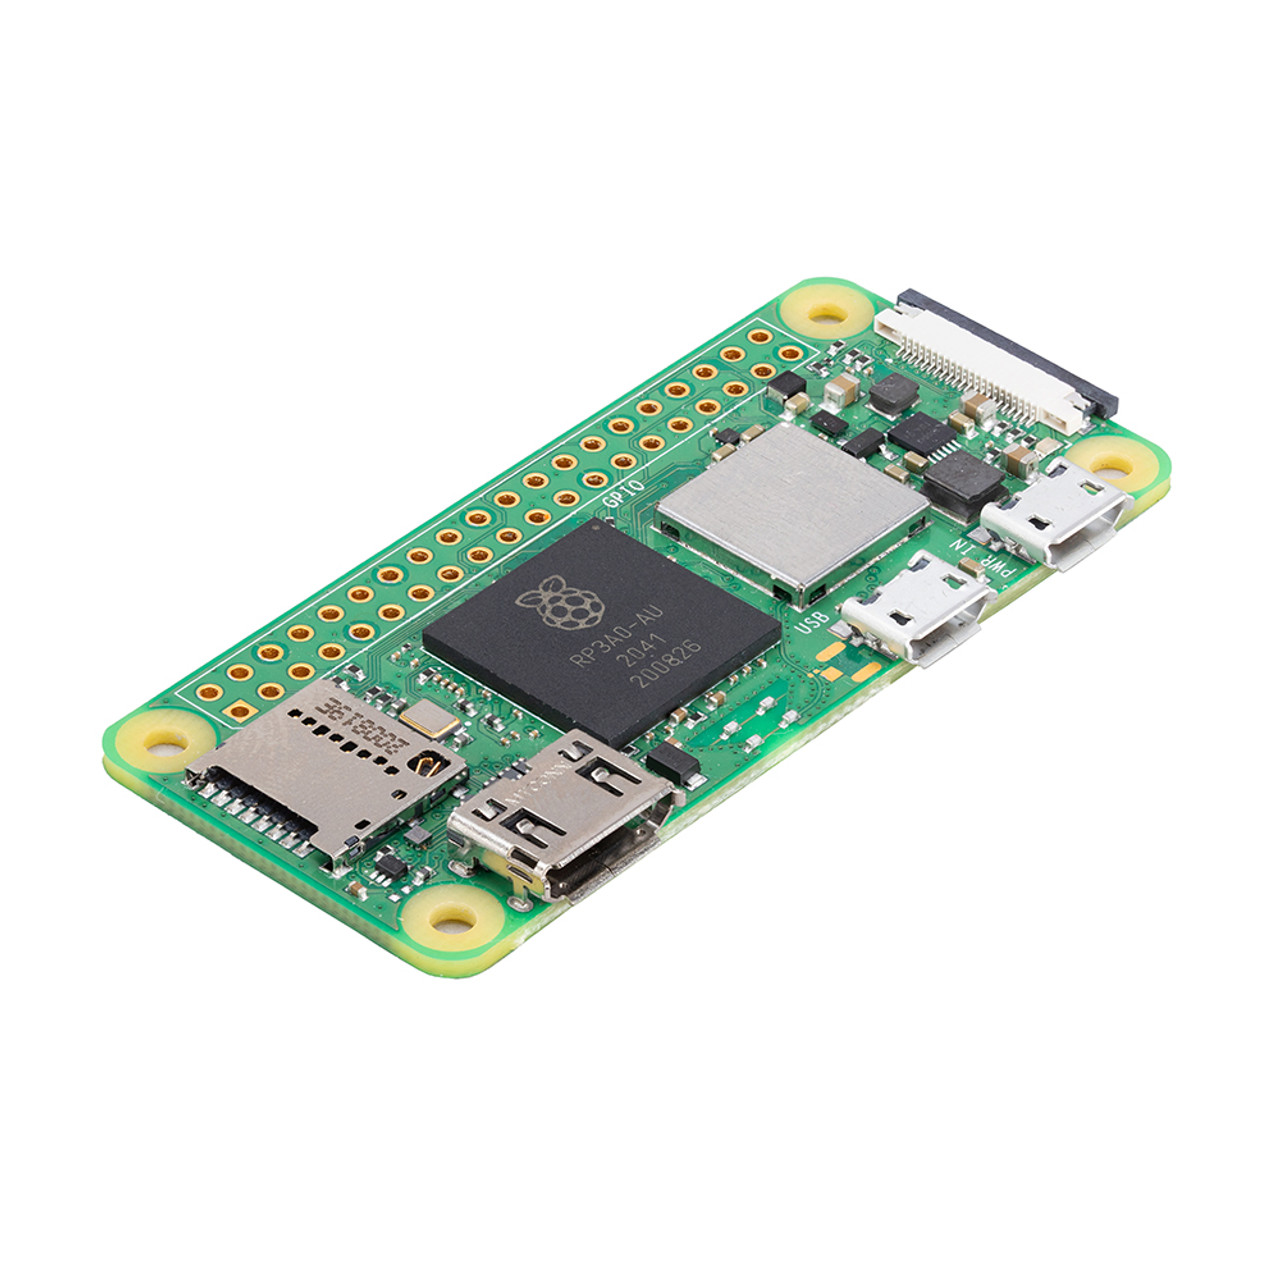
\includegraphics[width=0.3\textwidth]{Figures/PiZero_2.jpg}
    \caption{Raspberry Pi Zero 2 W}
    \label{fig:raspberrypi}
\end{figure}

\subsubsection{Camera App}

\begin{minipage}{\linewidth}
    We developed a \textbf{Python} application to display the live camera feed in a \textbf{Tkinter GUI} window,
    allowing the user to observe and record the operation of the robot. The user interface provided the ability to also
    take snapshots and store these in the \textbf{SD Card} storage. \\

    The live feed was largely a result of scheduling an update function with \textbf{Tkinter}'s \texttt{after(\dots)} method,
    which allowed us to sample camera frames at a rate of $20$ FPS. \\

    Since the \textbf{Raspberry Pi Zero 2 W} had power and performance constraints (i.e. $512$ MB of SDRAM),
    we ensured that the application was optimized for performance and iterated software versioning
    to minimize resource consumption. The camera was configured to capture frames at a resolution of $480$ pixels to account for this. \\
\end{minipage}

\begin{figure}[H]
    \centering
    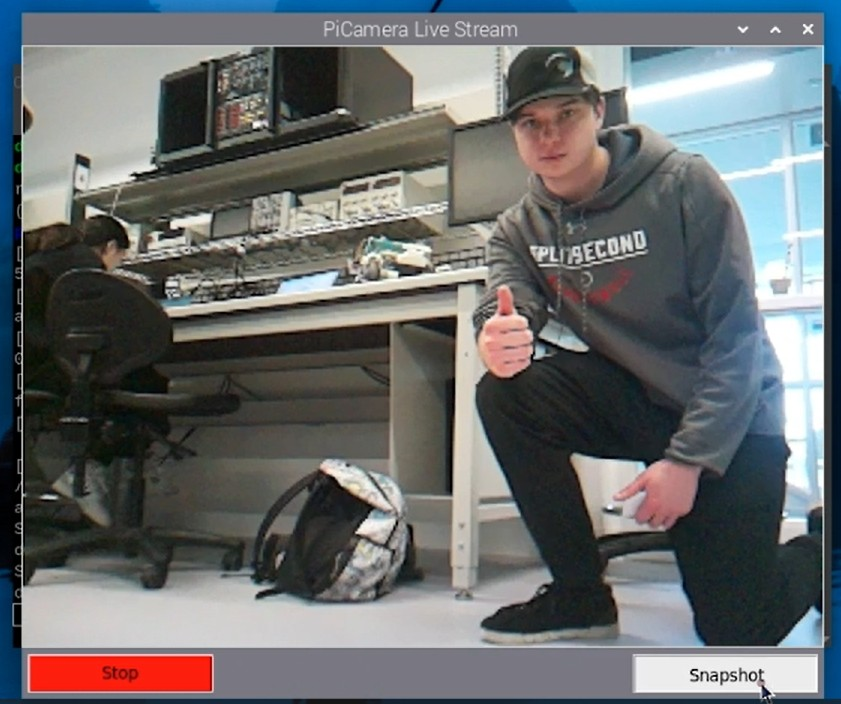
\includegraphics[width=0.5\textwidth]{Figures/PiCamera_App.jpg}
    \caption{PiCamera Application}
    \label{fig:camera_app}
\end{figure}

\begin{center}
    The class and methods for the camera display are shown in Listing \ref{lst:picamera_display_code} in the Appendix. \\
\end{center}


\begin{minipage}{\linewidth}
    Early on in development, we switched from the \textbf{Kivy} framework. This provided smoother animations, but rendering was
    hardware accelerated. We were unconfident with the \textbf{Raspberry Pi Zero 2 W}'s ability to provide adequate performance with this,
    and ported the application to the current implementation.
\end{minipage}

\subsubsection{AWS Bucket}

\begin{minipage}{\linewidth}
    Another constraint we considered during implementation was the inability to
    connect to the \textbf{Raspberry Pi} without powering on the robot. Having to access recording and snapshots
    would be quite cumbersome for the user. \\
\end{minipage}

\begin{figure}[H]
    \centering
    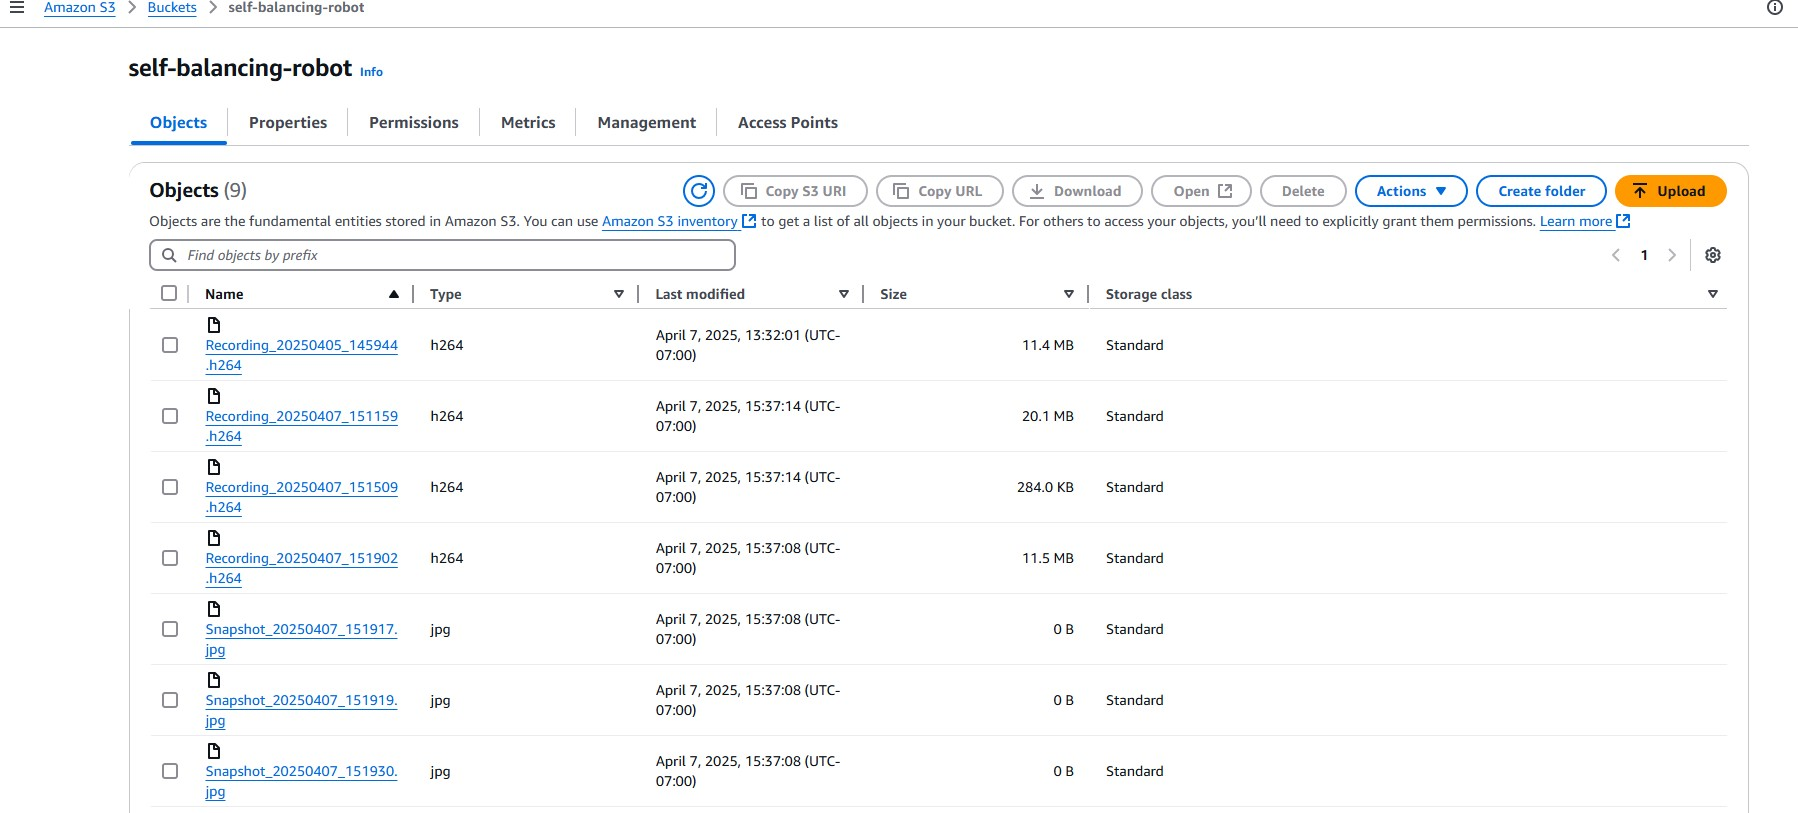
\includegraphics[width=1\textwidth]{Figures/S3Bucket_Files.jpg}
    \caption{AWS S3 Bucket}
    \label{fig:s3_bucket}
\end{figure}

\begin{minipage}{\linewidth}
    We created an \textbf{AWS S3 Bucket} and uploaded the camera recordings and snapshots during operation.
    The \textbf{Boto} package enabled us to implement this in our \textbf{Python} application by leveraging the \textbf{AWS SDK}.
    We were able to download these files from the \textbf{AWS S3 Bucket} to our local machine for offline access.
\end{minipage}

\section{Verification and Validation}
\subsection{Verification}
testing methods and results to demonstrate that the product meets the specified requirements. \\
\subsection{Validation}: Testing methods and results to demonstrate that the product actually will meet the high-level goals.

\section{Conclusions and Future Work}
Summary of the outcomes achieved/learned
Recommendations for next steps or further improvements


\section{References}
Cite any academic papers, industry standards, or prior work consulted in the project. Use consistent reference
formatting (e.g. https://pitt.libguides.com/citationhelp/ieee )


\section{Appendices}
Include sections that do not fit well in the main body of the report but help to show the development progress and justify your decisions. These might include (but may not be restricted to) the following:
\subsection{Appendix: Budget} (list all expenditures including any cost overrun)

\subsection{Appendix: Technical Calculations and Simulations}

\begin{table}[H]
    \centering
    \caption{IMU Sensors: Pros and Cons}
    \label{tab:imu_sensors}
    \begin{tabularx}{\textwidth}{|l|X|X|}
    \hline
    \textbf{Sensor} & \textbf{Pros} & \textbf{Cons} \\
    \hline
    \textbf{Accelerometer} &
    \begin{itemize}
        \item accurate gravitational readings
        \item zero-mean noise
    \end{itemize} &
    \begin{itemize}
        \item high noise variance (especially with motor vibrations)
    \end{itemize} \\
    \hline
    \textbf{Gyroscope} &
    \begin{itemize}
        \item lower noise over short time periods
    \end{itemize} &
    \begin{itemize}
        \item accumulates bias over time
    \end{itemize} \\
    \hline
    \end{tabularx}
\end{table}

\subsection{Appendix: Drawings, Schematics, and Blueprints}

\subsection{Appendix: Datasheets / Product Specifications}
Supporting Datasheets and Technical Documentation for Core Features (does not include battery related components, mechanical components, or generic electrical components):

\begin{enumerate}
    \item \href{https://docs.arduino.cc/resources/datasheets/ABX00069-datasheet.pdf}{Arduino Nano 33 IoT (ABX00069) Datasheet}
    \item \href{https://www.pololu.com/file/0J1736/pololu-37d-metal-gearmotors-rev-1-2.pdf}{Pololu 37D Metal Gearmotor Specifications}
    \item \href{https://www.ti.com/lit/ds/symlink/drv8833.pdf?ts=1743785858420}{Texas Instruments DRV8833 Dual H-Bridge Motor Driver Datasheet}
\end{enumerate}

\

Supporting Datasheets and Technical Documentation for Additional Features:
\begin{enumerate}
    \item \href{https://cdn.sparkfun.com/datasheets/Sensors/Proximity/HCSR04.pdf}{HC-SR04 Ultrasonic Distance Sensor}
    \item \href{https://cdn-shop.adafruit.com/datasheets/TCS34725.pdf}{TCS34725 Color Sensor}
    \item \href{https://datasheets.raspberrypi.com/rpizero2/raspberry-pi-zero-2-w-product-brief.pdf}{Raspberry Pi Zero 2 W}
    \item \href{https://mm.digikey.com/Volume0/opasdata/d220001/medias/docus/60/CN0090%20DATASHEET.pdf}{CN0090 Accelerometer Board}
    \item \href{https://www.st.com/content/ccc/resource/technical/document/datasheet/d3/84/d5/f6/3c/23/40/7b/CD00001883.pdf/files/CD00001883.pdf/jcr:content/translations/en.CD00001883.pdf}{L293D Motor Driver IC}
    \item \href{https://store.freenove.com/products/fnk0056}{Freenove 5MP Camera (FNK0056)}
    \item \href{https://www.sameskydevices.com/product/resource/cem-1203-42-.pdf?srsltid=AfmBOorbfJiXs7OIBQN95JLHokXYxTFx0Sd8qTPObMLqcfIHXVElk2uz}{CEM-1302 Speaker/Buzzer}
\end{enumerate}
\subsection{Appendix: Relevant Industry Standards and Regulations Used}

\subsection{Appendix: Prototypes}

\subsection{Appendix: Sample Code}

\begin{lstlisting}[caption={Arduino IMU Complementary Filter Firmware Implementation}, label={lst:arduino_angle_code}]
ANGLES Angles = {0, 0, 0}; // Accelerometer, Gyroscope, Complementary
void getAngles(ANGLES &Angles) {
  float currAccel, currGyro, currComplementary;
  float sampleTime;

  if (!IMU.gyroscopeAvailable()) return;
  IMU.readGyroscope(gx, gy, gz);

  if (!IMU.accelerationAvailable()) return;
  IMU.readAcceleration(ax, ay, az);

  currAccel = atan2(az, ay) * (180 / PI);
  currAccel = (currAccel - 90) + ACCELEROMETER_OFFSET;

  sampleTime = 1.0 / IMU.gyroscopeSampleRate();

  currGyro = prevGyro + gx * sampleTime;

  prevAngle = prevComplementary;
  currComplementary = k * (prevComplementary + gx * sampleTime) + (1 - k) * currAccel;

  /* Update Time Variables */
  t_n = millis(); // Current Time in Milliseconds
  dt = (t_n - t_n1) / 1000.0; // Time Difference in Seconds
  t_n1 = t_n; // Assign Current Time to Previous Time

  /* Update Angles */
  Angles.Accelerometer = currAccel;
  Angles.Gyroscope = currGyro;
  Angles.Complementary = currComplementary;

  /* Assign Previous Angles */
  prevGyro = currGyro;
  prevComplementary = currComplementary;
}
\end{lstlisting}

\begin{lstlisting}[caption={STM32 HC-SR04 Firmware Implementation}, label={lst:stm32_distancesensor_code}]
void DistanceSensor_InputCaptureInterrupt(distancesensor* sensor)
{
    if (HAL_GPIO_ReadPin(sensor->icGPIOPort, sensor->icGPIOPin)) {
        sensor->IC_Value1 = HAL_TIM_ReadCapturedValue(sensor->timer, TIM_CHANNEL_1); // First rising edge
        HAL_TIM_PWM_Stop(sensor->timer, TIM_CHANNEL_2);
    }
    else {
        sensor->IC_Value2 = HAL_TIM_ReadCapturedValue(sensor->timer, TIM_CHANNEL_1); // Second rising edge
        if (sensor->IC_Value2 > sensor->IC_Value1) {
            sensor->timeDifference = sensor->IC_Value2 - sensor->IC_Value1;
        }
        else {
            sensor->timeDifference = (TIM_PERIOD + 1 - sensor->IC_Value1) + sensor->IC_Value2; // Handle overflow
        }

        HAL_TIM_PWM_Start(sensor->timer, TIM_CHANNEL_2);
        __HAL_TIM_SetCounter(sensor->timer, 65535);

        DistanceSensor_Handle(sensor);
    }
}

// On main.c:

void HAL_TIM_IC_CaptureCallback(TIM_HandleTypeDef *htim) {
    if (htim->Instance == TIM21) {
		DistanceSensor_InputCaptureInterrupt(&Front);
	}
	else if (htim->Instance == TIM22) {
		DistanceSensor_InputCaptureInterrupt(&Back);
	}

}
\end{lstlisting}



\begin{lstlisting}[caption={STM32 TCS34725 Firmware Implementation}, label={lst:stm32_colorsensor_code}]
#include "colorsensor.h"

#define TCS3472_SLAVE_ADDRESS 0x29 << 1
#define TCS3472_EXPECTED_ID 0x44

#define TCS3472_ID_REG 0x12

#define TCS3472_WTIME_REG 0x03
#define TCS3472_ATIME_REG 0xF6
#define TCS3472_ENABLE_REG 0x00

#define TCS3472_CDATAL_REG 0x14
#define TCS3472_RDATAL_REG 0x16
#define TCS3472_GDATAL_REG 0x18
#define TCS3472_BDATAL_REG 0x1A

extern speaker Speaker;

void ColorSensor_Init(colorsensor* sensor, I2C_HandleTypeDef* i2c_handle) {
    sensor->i2c = i2c_handle;
    sensor->slave_address = TCS3472_SLAVE_ADDRESS;

    memset(sensor->rgb_data, 0, sizeof(sensor->rgb_data));  // Clear RGB data
    sensor->enabled = true;
    sensor->count = 0;

    // Define initialization sequence
    uint8_t init_data[][2] = {
        { TCS3472_WTIME_REG  | 0x80, 0xFF },  // Wait time
        { TCS3472_ATIME_REG  | 0x80, 0xFF },  // Integration time
        { TCS3472_ENABLE_REG | 0x80, 0x0B },   // Power ON & enable RGBC
    };

    // Loop through initialization commands and send them
    for (size_t i = 0; i < sizeof(init_data) / sizeof(init_data[0]); i++) {
        if (HAL_I2C_Master_Transmit(sensor->i2c, sensor->slave_address, init_data[i], 2, HAL_MAX_DELAY) != HAL_OK)
        	while(1);
    }

    HAL_GPIO_WritePin(COLOR_SENSOR_STATUS_GPIO_Port, COLOR_SENSOR_STATUS_Pin, GPIO_PIN_SET);
}


void ColorSensor_EnableStatus(colorsensor* sensor, bool enable)
{
	sensor->enabled = enable;
}


uint16_t ColorSensor_Read16(colorsensor* sensor, uint8_t reg) {
    uint8_t buffer[2];
    uint8_t command = reg | 0xA0;  // Add auto-increment bit

    // Send register address
    if (HAL_I2C_Master_Transmit(sensor->i2c, sensor->slave_address, &command, 1, HAL_MAX_DELAY) != HAL_OK) {
        return 0; // Handle error
    }

    // Read 2 bytes from the sensor
    if (HAL_I2C_Master_Receive(sensor->i2c, sensor->slave_address, buffer, 2, HAL_MAX_DELAY) != HAL_OK) {
        return 0; // Handle error
    }

    // Combine two bytes into a 16-bit value (LSB first)
    return (uint16_t)(buffer[0] | (buffer[1] << 8));
}

void ColorSensor_ReadAll(colorsensor* sensor) {
    sensor->rgb_data[0] = ColorSensor_Read16(sensor, TCS3472_CDATAL_REG); // TCS3472_CDATAL
    sensor->rgb_data[1]   = ColorSensor_Read16(sensor, TCS3472_RDATAL_REG); // TCS3472_RDATAL
    sensor->rgb_data[2] = ColorSensor_Read16(sensor, TCS3472_GDATAL_REG); // TCS3472_GDATAL
    sensor->rgb_data[3]  = ColorSensor_Read16(sensor, TCS3472_BDATAL_REG); // TCS3472_BDATAL
}


color ColorSensor_CalculateColor(colorsensor* sensor)
{
	uint16_t max_val = sensor->rgb_data[1];
	color detected_color = RED;

	if (sensor->rgb_data[2] > max_val) detected_color = GREEN;
	if (sensor->rgb_data[3] > max_val) detected_color = BLUE;

	return detected_color;
}

void ColorSensor_Handle(colorsensor* sensor)
{
	ColorSensor_ReadAll(sensor);
	color detected_color = ColorSensor_CalculateColor(sensor);

	if (detected_color == RED)
	{
		HAL_GPIO_WritePin(COLOR_SENSOR_STATUS_GPIO_Port, COLOR_SENSOR_STATUS_Pin, GPIO_PIN_RESET);
		if (!Speaker.hasFault)
			Speaker_Start(&Speaker, COLOR_SENSOR_ID);
	}
	else
	{
		HAL_GPIO_WritePin(COLOR_SENSOR_STATUS_GPIO_Port, COLOR_SENSOR_STATUS_Pin, GPIO_PIN_SET);
		if (Speaker.hasFault)
			Speaker_Stop(&Speaker, COLOR_SENSOR_ID);
	}


}
\end{lstlisting}

\begin{lstlisting}[caption={STM32 RC522 Firmware Implementation}, label={lst:stm32_rfidsensor_code}]
#include "rfid.h"

#include "speaker.h"

#define SERIALNUM_1_IDLE 32

#define SERIALNUM_0_CORRECT_CARD 170
#define SERIALNUM_1_CORRECT_CARD 205
#define SERIALNUM_2_CORRECT_CARD 47
#define SERIALNUM_3_CORRECT_CARD 3
#define SERIALNUM_4_CORRECT_CARD 75

extern speaker Speaker;
extern UART_HandleTypeDef huart1;
extern char Data;

void RFID_Init(rfid* sensor) {
    MFRC522_Init();
    memset(sensor->prevSerialNum, 0, 5);
    sensor->status = CARD_IDLE;

    sensor->botEnabled = false;
    sensor->initialSuccessfulCardTap = true;
    sensor->initialFailedCardTap = true;

    HAL_GPIO_WritePin(RFID_STATUS_GPIO_Port, RFID_STATUS_Pin, GPIO_PIN_SET);
}

rfid_card_status RFID_ValidateCard(rfid* sensor)
{
	uint8_t serialNum[5];
	MFRC522_Request(PICC_REQIDL, serialNum);
	MFRC522_Anticoll(serialNum);

	sensor->status = CARD_IDLE;

	if ((serialNum[0] == 170 && serialNum[1] == 205 && serialNum[2] == 47 && serialNum[3] == 3 && serialNum[4] == 75) ||
			(sensor->prevSerialNum[0] == 170 && sensor->prevSerialNum[1] == 205 && sensor->prevSerialNum[2] == 47 && sensor->prevSerialNum[3] == 3 && sensor->prevSerialNum[4] == 75))
	{
		sensor->status = CARD_SUCCESS;

	}
	else if (!(serialNum[0] | (!(serialNum[1] == 32 || serialNum[1] == 0)) | serialNum[2] | serialNum[3] | serialNum[4]))
	{
		if (!(sensor->prevSerialNum[0] | sensor->prevSerialNum[1] | sensor->prevSerialNum[2] | sensor->prevSerialNum[3] | sensor->prevSerialNum[4]))
			sensor->status = CARD_IDLE;
		else
		{
			sensor->status = CARD_FAIL;
		}

	}
	else
	{
		sensor->status = CARD_FAIL;
	}


	for (uint8_t i = 0; i < 5; i++)
	{
		sensor->prevSerialNum[i] = serialNum[i];
	}

	return sensor->status;
}

void RFID_SecurityLogic(rfid* sensor)
{
	rfid_card_status cardStatus = RFID_ValidateCard(sensor);

	switch (cardStatus) {
	    case CARD_SUCCESS:
	    	if (sensor->initialSuccessfulCardTap)
	    	{

	    		Speaker_SetAutoReload(&Speaker, 488);
	    		Speaker_Beep(&Speaker, 150, 0, 1);
	    		sensor->initialSuccessfulCardTap = false;
	    		sensor->initialFailedCardTap = true;
	    		sensor->botEnabled = !sensor->botEnabled;
	    		HAL_GPIO_WritePin(RFID_STATUS_GPIO_Port, RFID_STATUS_Pin, (GPIO_PinState) !sensor->botEnabled);
	    	}
	        break;

	    case CARD_FAIL:
	    	if (sensor->initialFailedCardTap)
	    	{
	    		HAL_Delay(200);
				if (RFID_ValidateCard(sensor) != CARD_FAIL)
					break;
				Speaker_SetAutoReload(&Speaker, 488 * 4);
				Speaker_Beep(&Speaker, 150, 50, 4);
				sensor->initialSuccessfulCardTap = true;
				sensor->initialFailedCardTap = false;


	    	}
	        break;

	    case CARD_IDLE:
	    	sensor->initialSuccessfulCardTap = true;
	    	sensor->initialFailedCardTap = true;
	        break;

	    // Optional: Default case if no case matches
	    default:
	        // Code to execute if none of the above cases match
	        break;
	}

}

\end{lstlisting}

\begin{lstlisting}[caption={STM32 Speaker Firmware Implementation}, label={lst:stm32_speaker_code}]
#include "speaker.h"


#define CLK_SPEED 32000000
#define DEFAULT_AUTORELOAD 488

void Speaker_Init(speaker* speaker, rfid* rfid_struct, TIM_HandleTypeDef* timer)
{
	speaker->rfid_sensor = rfid_struct;
	speaker->timer = timer;

	speaker->hasFault = false;
	speaker->beepLengthOn = 0;
	speaker->beepLengthPeriod = 0;
	speaker->wantedNumBeeps = 0;
	speaker->currentNumBeeps = 0;
	speaker->timerCounter = 0;

	for (uint8_t i = 0; i < sizeof(speaker->featureFault) / sizeof(speaker->featureFault[0]); i++)
	{
		speaker->featureFault[i] = false;
	}


}

void Speaker_Start(speaker* speaker, uint8_t ID)
{

	speaker->featureFault[ID] = true;
	if ((speaker->featureFault[0] || speaker->featureFault[1] || speaker->featureFault[2]) && speaker->rfid_sensor->botEnabled)
	{
		speaker->hasFault = true;
		Speaker_SetAutoReload(speaker, DEFAULT_AUTORELOAD);
		HAL_TIM_PWM_Start(speaker->timer, TIM_CHANNEL_1);
	}

}

void Speaker_Stop(speaker* speaker, uint8_t ID)
{
	speaker->featureFault[ID] = false;
	if (!(speaker->featureFault[0] || speaker->featureFault[1] || speaker->featureFault[2]))
	{
		speaker->hasFault = false;
		HAL_TIM_PWM_Stop(speaker->timer, TIM_CHANNEL_1);
	}
}



bool Speaker_Beep(speaker* speaker, uint16_t length_on_ms, uint16_t length_off_ms, uint8_t numBeeps)
{

	if (speaker->hasFault)
		return false;


	speaker->timerCounter = 0;
	speaker->currentNumBeeps = 0;



	speaker->beepLengthOn = length_on_ms * 1000 / __HAL_TIM_GET_AUTORELOAD(speaker->timer);
	speaker->beepLengthPeriod =speaker->beepLengthOn + length_off_ms * 1000 / __HAL_TIM_GET_AUTORELOAD(speaker->timer);
	speaker->wantedNumBeeps = numBeeps;

	//speaker->beepLength = length_ms * CLK_SPEED / (speaker->timer->Instance->PSC);

	HAL_TIM_Base_Start_IT(speaker->timer);
	HAL_TIM_PWM_Start(speaker->timer, TIM_CHANNEL_1);
	return true;
}

void Speaker_BeepInterrupt(speaker* speaker)
{
    if (speaker->currentNumBeeps < speaker->wantedNumBeeps)
    {

        if (speaker->timerCounter == speaker->beepLengthOn)
        {
            HAL_TIM_PWM_Stop(speaker->timer, TIM_CHANNEL_1);
            __HAL_TIM_ENABLE(speaker->timer);
        }
        else if (speaker->timerCounter >= speaker->beepLengthPeriod)
        {
        	speaker->currentNumBeeps++;
			speaker->timerCounter = 0;

            if (speaker->currentNumBeeps < speaker->wantedNumBeeps)
            {
                HAL_TIM_PWM_Start(speaker->timer, TIM_CHANNEL_1);

            }

        }
        speaker->timerCounter++;
    }
    else
    {
        HAL_TIM_PWM_Stop(speaker->timer, TIM_CHANNEL_1);
        HAL_TIM_Base_Stop_IT(speaker->timer);
    }
}

void Speaker_SetAutoReload(speaker* speaker, uint16_t value)
{
	__HAL_TIM_SET_AUTORELOAD(speaker->timer, value);
	__HAL_TIM_SET_COMPARE(speaker->timer, TIM_CHANNEL_1, value / 2);
}

\end{lstlisting}

\begin{lstlisting}[caption={Robot Driver App}, label={lst:driver_app_code}]
    import asyncio
    import threading

    from bleak import BleakScanner, BleakClient, BleakError
    from flask import Flask, request, jsonify, render_template

    class BLEManager:
        # Define UUIDs for BLE Service and Characteristic
        SERVICE_UUID = "00000000-5EC4-4083-81CD-A10B8D5CF6EC"
        CHARACTERISTIC_UUID = "00000001-5EC4-4083-81CD-A10B8D5CF6EC"
        CODE = "0095" # Authentication Code

        def __init__(self):
            self.devices = []
            self.client = None
            self.is_connected = False

            self.loop = asyncio.new_event_loop()
            self.start_loop()

        def start_loop(self):
            threading.Thread(target = self._run_loop, daemon = True).start()

        def _run_loop(self):
            asyncio.set_event_loop(self.loop)
            self.loop.run_forever()

        def run_async(self, coro):
            return asyncio.run_coroutine_threadsafe(coro, self.loop)

        async def scan_devices(self):
            self.devices = []
            scanned = await BleakScanner.discover()

            self.devices = [
                {"name" : device.name, "address" : device.address} for device in scanned if device.name and ("WALL-E" in device.name)
            ] # Filter BLE Devices
            return self.devices

        async def connect_device(self, address):
            """Connect to BLE Device."""
            if self.client and self.client.is_connected:
                self.is_connected = True
                return True

            self.client = BleakClient(address)
            try:
                await self.client.connect()
                await self.client.write_gatt_char(BLEManager.CHARACTERISTIC_UUID, BLEManager.CODE.encode("utf-8"))
                self.is_connected = self.client.is_connected
                return self.is_connected
            except BleakError:
                self.is_connected = False
                return False

        async def disconnect_device(self):
            """Disconnect from BLE Device."""
            if self.client and self.client.is_connected:
                await self.client.disconnect()
            self.is_connected = False

        async def send_cmd(self, cmd):
            """Schedule Send Command Coroutine Using Button's Custom Command."""
            if not (self.client and self.client.is_connected):
                return False, "Not Connected to BLE"
            try:
                await self.client.write_gatt_char(BLEManager.CHARACTERISTIC_UUID, cmd.encode("utf-8"))
                return True, f"Sent Command: {cmd}"
            except BleakError as e:
                return False, f"Error Sending Command: {e}"

    class RobotDriverApp:
        def __init__(self):
            self.app = Flask("Robot Driver App")
            self.ble_manager = BLEManager()
            self._register_routes()

        def _register_routes(self):
            @self.app.route("/")
            def index():
                return render_template("index.html")

            @self.app.route("/scan", methods = ["GET"])
            def scan():
                future = self.ble_manager.run_async(self.ble_manager.scan_devices())
                devices = future.result(timeout = 30) # Wait for 30 Seconds
                return jsonify(devices)

            @self.app.route("/connect", methods = ["POST"])
            def connect():
                data = request.get_json()
                if not data or "deviceAddress" not in data:
                    return jsonify({"error": "No Address Provided"}), 400
                future = self.ble_manager.run_async(self.ble_manager.connect_device(data["deviceAddress"]))
                success = future.result(timeout = 15) # Wait for 15 Seconds
                return (jsonify({"status": "Connected"}) if success
                        else (jsonify({"status": "Failed"}), 400))

            @self.app.route("/disconnect", methods = ["GET"])
            def disconnect():
                future = self.ble_manager.run_async(self.ble_manager.disconnect_device())
                future.result(timeout = 10) # Wait for 5 Seconds
                return jsonify({"status": "Disconnected"})

            @self.app.route("/move", methods = ["POST"])
            def move():
                data = request.get_json()
                if not data or "command" not in data:
                    return jsonify({"error": "No Command Provided"}), 400 # Bad Request

                future = self.ble_manager.run_async(
                    self.ble_manager.send_cmd(data["command"])
                )
                success, message = future.result(timeout = 10) # Wait for 5 Seconds

                if success:
                    return jsonify({"status": "OK", "msg": message})
                else:
                    return jsonify({"status": "Error", "msg": message}), 400 # Bad Request

        def run(self):
            self.app.run(host = "0.0.0.0", port = 5000, debug = False)

    if __name__ == "__main__":
        RobotDriverApp().run()
\end{lstlisting}


\begin{lstlisting}[caption={PiCamera Display}, label={lst:picamera_display_code}]
from picamera2 import Picamera2
from picamera2.encoders import H264Encoder
from libcamera import Transform

class CameraDisplay(tk.Frame):
    SAMPLE_RATE = 1.0 / 50.0 # Update Delay ~20 FPS (1000ms/20 = 50ms)
    def __init__(self, parent, *args, **kwargs):
        super().__init__(parent, *args, **kwargs)

        self.filename = ""
        self.camera = Picamera2() # Init Camera

        self.snapshot_dir: str = os.path.join(os.path.dirname(os.path.abspath(__file__)), "Snapshots")
        self.video_dir: str = os.path.join(os.path.dirname(os.path.abspath(__file__)), "Videos")

        os.makedirs(self.snapshot_dir, exist_ok = True)
        os.makedirs(self.video_dir, exist_ok = True)

        # Force RGB888 Output
        self.config = self.camera.create_video_configuration(
            main = {
                "size": (640, 480), # Default Size
                # "size": (1280, 720), # HD
                # "size": (1920, 1080), # Full HD
                "format": "RGB888"
            },
            transform = Transform(hflip = False, vflip = False) # For Tkinter Display
        )
        self.image_label = tk.Label(self)
        self.image_label.pack()

    def start_recording(self):
        self.camera.configure(self.config)
        self.camera.start()

        self.filename = f"Recording_{dt.datetime.now().strftime('%Y%m%d_%H%M%S')}"
        input_file = os.path.join(self.video_dir, f"{self.filename}.h264")

        self.camera.start_recording(H264Encoder(bitrate = 10000000), input_file)

    def stop_recording(self):
        if self.filename == "":
            return

        self.camera.stop_recording()
        self.camera.stop()
        self.filename = ""

    def take_snapshot(self):
        if self.filename == "":
            self.camera.configure(self.config)
            self.camera.start()

        # Capture Current Frame
        frame = self.camera.capture_array()
        if frame is None or frame.size == 0:
            print("Failed to Capture Snapshot.")
            return

        # Swap Color Channels (BGR -> RGB)
        frame = frame[..., ::-1]

        snapshot_name = f"Snapshot_{dt.datetime.now().strftime('%Y%m%d_%H%M%S')}.jpg"
        snapshot_path = os.path.join(self.snapshot_dir, snapshot_name)

        # Convert to PIL Image
        image = PILImage.fromarray(frame)
        image.save(snapshot_path) # Save Image
        print(f"Snapshot Saved to {snapshot_path}")

        if self.filename == "":
            self.camera.stop()

    def update(self):
        if self.filename == "":
            return

        frame = self.camera.capture_array()
        if (frame is not None) and (frame.size != 0):
            frame = frame[..., ::-1] # BGR -> RGB

            # Convert the PIL Image to an ImageTk.PhotoImage
            self.image_label.current = ImageTk.PhotoImage(
                image = PILImage.fromarray(frame) # Convert Numpy Array to PIL.Image
            )
            self.image_label.configure(image = self.image_label.current)

    def stop(self):
        self.camera.close()
\end{lstlisting}

\end{document}
